\documentclass[11.5pt]{sig-alternate} % sets document style to sig-alternate
% packages
% typesetting
%\usepackage{dirtytalk} % typset quotations easier (\say{stuff})
\usepackage{hanging} % hanging paragraphs
\usepackage[defaultlines=3,all]{nowidow} % avoid widows
\usepackage[pdfpagelabels=false]{hyperref} % produce hypertext links, includes backref and nameref
\usepackage{xurl} % defines url linebreaks, loads url package
\usepackage{microtype}
\usepackage{textgreek}
%\usepackage{textcomp}
%\newcommand{\texttildemid}{\raisebox{0.4ex}{\texttildelow}}
% layout
\usepackage{enumitem} % control layout of itemize, enumerate, description
\usepackage{fancyhdr} % control page headers and footers
\usepackage{float} % improved interface for floating objects
%\usepackage{multicol} % intermix single and multiple column pages
% language
\usepackage[utf8]{inputenc} % accept different input encodings
\usepackage[english]{babel} % multilanguage support
% misc
\usepackage{graphicx} % builds upon graphics package, \includegraphics
%\usepackage{lastpage} % reference number of pages
%\usepackage{comment} % exclude portions of text (?)
\usepackage{xcolor} % color extensions
\usepackage[backend=biber, style=apa]{biblatex} % sophisticated bibliographies % necessary for HTML to display author info and date on abstract page
\usepackage{csquotes} % advanced quotations, makes biblatex happy
\usepackage{authblk} % support for footnote style author/affiliation
% tables and figures
\usepackage{tabularray}
%\usepackage{array} % extend array and tabular environments
\usepackage{caption} % customize captions in figures and tables (rotating captions, sideways captions, etc)
%\usepackage{cuted} % allow mixing of \onecolumn and \twocolumn on same page
\usepackage{multirow} % create tabular cells spanning multiple rows
%\usepackage{subfigure} % deprecated, support for manipulation of small figures
%\usepackage{tabularx} % extension of tabular with column designator "x", creates paragraph-like column whose width automatically expands
%\usepackage{wrapfig} % allows figures or tables to have text wrapped around them
%\usepackage{booktabs} % better rules
% dummy text
%\usepackage{blindtext} % blind text dummy text
%\usepackage{kantlipsum} % Kant style dummy text
\usepackage{lipsum} %lorem ipsum dummy text
% other helpful packages may be booktabs, longtable, longtabu, microtype

\pagestyle{fancy} % sets pagestyle to fancy for fancy headers and footers

% header and footer
% modern way to set header image
\renewcommand{\headrulewidth}{0pt} % defines thickness of line under header
\renewcommand{\footrulewidth}{0pt} % defines thickness of line above header
\setlength\headheight{80.0pt} % sets height between top margin and header image, effectively moves page contents down
\addtolength{\textheight}{-80.0pt} % seems to affect the lower height. maybe only works properly if footer numbers enabled?
\fancyhf{}
\fancyhead[CE, CO]{
\includegraphics[width=\textwidth]{headerImage.png}}
% footer
%\fancyfoot[LE,LO]{Article Title Here \\ DOI: }% left footer article title and doi
%\fancyfoot[CE,CO]{{}} % center footer empty
%\fancyfoot[RE,RO]{\thepage} % right footer page numbers
%\pagenumbering{arabic} % arabic (1, 2, 3) numbering in footer

\hypersetup{colorlinks=true,urlcolor=blue} % sets link color to blue
\urlstyle{same} % sets url typeface to same as rest of text

% set caption and figure to italics, label bold, left align captions, does not transfer to HTML
\captionsetup{labelfont=bf, font={large, it}, justification=raggedright, singlelinecheck=false}
\renewcommand\theContinuedFloat{\alph{ContinuedFloat}}

%this next bit is confusing, but essentially changes the width of the abstract. Seems to have been copied from this https://tex.stackexchange.com/questions/151583/how-to-adjust-the-width-of-abstract
\let\oldabstract\abstract
\let\oldendabstract\endabstract
\makeatletter %changes @ catcode to enable modification (in parsep)
\renewenvironment{abstract} %alters the abstract environment
{\renewenvironment{quotation}%
               {\list{}{\addtolength{\leftmargin}{1em} % change this value to add or remove length to the the default ?
                        \listparindent 1.5em%
                        \itemindent    \listparindent%
                        \rightmargin   \leftmargin%
                        \parsep        \z@ \@plus\p@}%
                \item\relax}%
               {\endlist}%
\oldabstract}
{\oldendabstract}
\makeatother %changes @ catcode to disable modification

% checks
% italics -
% links -
% dashes -
% tildes -
\begin{document}

\title{Signs of Autonomy: Facilitating Independence and Inquiry in Deaf Science Classrooms}

\author[1]{\large \color{blue}Sami Kahn}
\author[1]{\large \color{blue}Allan Feldman}
\author[2]{\large \color{blue}Michele L. Cooke}

\affil[1]{University of South Florida}
\affil[2]{University of Massachusetts}

\toappear{}
%% ABSTRACT
\maketitle
\begin{@twocolumnfalse} 
\begin{abstract}
\item 
\textit{Deaf and hard of hearing (DHH) persons are underrepresented in the fields of science, technology, engineering, and mathematics (STEM). One of the major barriers to STEM careers is DHH students’ extremely low college graduation rates. While social and literacy barriers play a critical role in this phenomenon, student autonomy has also been cited as a major contributor. DHH students have been characterized as dependent learners, a learning style possibly reinforced by reliance on adults for disproportionate amounts of information, as well as a tendency of deaf educators to teach in highly structured, explicit manners. Dependent learning styles can impede autonomy at the college level and also run counter to current conceptualizations of scientific inquiry. For DHH students to succeed in science, they must develop habits of mind consistent with those of practicing scientists and demonstrate high levels of inquiry. This study utilized frameworks of learning style and science inquiry to identify the salient features of autonomy and inquiry in deaf science classrooms with the goal of isolating pedagogical strategies to foster these skills. Applying a general inductive approach, this instrumental cross-case study looks at three earth science classrooms located in three high schools for deaf students. Videos of instructional periods were taken and analyzed for each classroom. Findings suggest that teacher facilitation of inquiry plays a major role in DHH students’ apparent learning style and ability to negotiate scientific problem-solving. A model describing teacher facilitation of autonomy and inquiry is developed and recommendations for fostering inquiry and autonomy are identified.}
\\ \\
\end{abstract}
\end{@twocolumnfalse}

%% AUTHOR INFORMATION

\textbf{*Corresponding Author,Sami Kahn }\\
\href{mailto: msamikahn@mail.usf.edu}{(samikahn@mail.usf.edu)} \\
\textit{Submitted Dec 18 2013 }\\
\textit{Accepted Dec 18 2013} \\
\textit{Published online Dec 19 2013 } \\
\textit{DOI:10.14448/jsesd.06.0001} \\
\pagebreak
\clearpage
\begin{large}
\section*{INTRODUTION}
Deaf and hard of hearing (DHH) persons are underrepresented in science, technology, engineering, and mathematics (STEM) careers (National Science Foundation, 2004).   This is attributable, in part, to the fact that only approximately 25\% of deaf students entering higher education graduate (Stinson \& Walter, 1997).  Social and literacy barriers (Lang \& Stinson, 1982), as well as issues of student autonomy including advocacy skills and independent decision-making ability (Scherer \& Walter, 1988) contribute to low graduation rates. Further, DHH students have been characterized as “dependent learners” (Lang, Stinson, Kavanaugh, Liu, \& Basile, 1999); that is, they rely heavily on teachers’ guidance in how and what they learn. While dependent learning styles are not unique to DHH students (Marschark, Lang, \& Albertini, 2002), learner dependence may be reinforced by deaf students’ required reliance on adults for communication and interpretation, a lack of opportunities for “unstructured play,” barriers to information that would otherwise be integrated from other sources, including media and friendships (McIntosh, Sulzen,  Reeder,  \& Kidd, 1994, p. 482), as well as deaf educators’ tendencies to teach in a very structured and explicit manner (Livingston, 1997; Enns, 2009).  Lang (2002) identified several key qualities that can foster success for deaf students in higher education, including self/career awareness, persistence, self-efficacy, and perseverance (p. 269), as well as the ability to advocate for interpreting, tutoring, and note-taking services. These traits are related to student autonomy, which is characterized by volitional and self-directed behaviors (Niemiec \& Ryan, 2009), and appear to be more closely aligned with independent or participative learning styles described by Grasha (1996). 

Evidence supports the notion that teachers can best educate students by teaching to their students’ “learning style” (Dunn \& Bruno, 1985; Foriska, 1992; Okebukola, 1986; Sternberg, Grigorenko, \& Zhang, 2008 ).  This implies that teacher-dependent learners would benefit from explicit direction and guidance to foster learning (Grasha, 1996).  However, this approach appears in conflict with the tenets of scientific inquiry, which are based on open exploration, student-driven questioning and determination of problems, and teacher as facilitator rather than information giver (Linn, Davis, \& Bell, 2004). This begs the question of how students who are dependent learners can ever gain autonomy, a necessary skill needed for both success in science and in higher learning, if teachers teach to their dependent style. This question needs to be considered if we are going to reconcile the theoretical gap between dependent learning and the need for autonomous thinking and decision-making required for success in higher education and STEM careers.

The purpose of this study is to explore the linkage between scientific inquiry teaching and the development of student autonomy and inquiry in DHH classes guided by the following research questions: 
\begin{enumerate}
    \item How does teachers’ facilitation of inquiry-based science teaching promote students’ inquiry experiences in a deaf science class?
    \item What are the signs of student autonomy in a deaf science class?
    \item How does the implementation of inquiry-based learning relate to student autonomy in a deaf science class?
\end{enumerate}
In responding to these research questions through cross-case methodology, this study sheds light on the relationships between inquiry and autonomy in a deaf science classroom, with emphasis on the effect of teacher facilitation on each.  

\section*{DHH STUDENTS IN THE SCIENCE CLASSROOM: CONNECTIONS BETWEEN INQUIRY AND AUTONOMY}

Learning styles refer to, “the manner in which individuals choose to or are inclined to approach a learning situation” (Cassidy, 2004, p.420). Grasha (1996) defines learning styles as “preferences students have for thinking, relating to others, and particular types of classroom environments and experiences” (p. 23-24.)  Using the Grasha-Riechmann Student Learning Styles Scales (GRS\\LSS), Lang, Stinson, Kavanaugh, Liu, \& Basile (1999) reported that DHH college students were found to be ‘‘dependent’’ learners, defined as students who rely on authority figures for guidelines and answers rather than formulating their own ideas,  thus making it “difficult to develop skills for exhibiting . . . self-direction as a learner’’ (p. 169).  While it has been suggested that dependent learners learn best when material is presented in an organized and structured manner (Grasha, 1996), perpetuating a dependent learning style through highly ordered instruction may not be conducive to success in higher education, which requires:  (a) developing social skills, (b) establishing an identity, and (c) acquiring independence and interdependence (Stinson \& Walter, 1997).  Failure to become independent or autonomous in information gathering or decision-making creates barriers for DHH students in higher education in general and in STEM careers specifically, due to the nature of scientific inquiry. 

In articulating their vision for K-12 education in natural sciences and engineering, the authors of the Frameworks for Science Education (National Research Council, 2012) cited the importance of preparing students to engage in scientific practices, including investigating, modeling, critiquing, and communicating.  This  view of science inquiry challenges students to take on the roles of scientists in authentic learning situations and challenges teachers to move curriculum beyond ‘cookbook’ approaches by providing opportunities for scientific reasoning and conceptual change (Bybee \& Van Scotter, 2007).  Linn, et al. (2004) defined inquiry in science as the “intentional process of diagnosing problems, critiquing experiments, and distinguishing alternatives, planning investigations, researching conjectures, searching for information, constructing models, debating with peers, and forming coherent arguments” (p. 16). This view of science inquiry can be distinguished from traditional curriculum in its emphasis on students moving along a continuum from being passive receivers of information to “self-directed learners” (Anderson, 2002, p. 5). Characteristics of such learners include designing their own activities and directing their own learning tasks, thereby exhibiting student autonomy which is characterized by volitional and self-determined behaviors (Niemiec \& Ryan, 2009). Science, as a discipline, requires certain “habits of mind” in order to fully access scientific inquiry.  Some of these characteristics include curiosity, honesty, openness, skepticism, persistence, and the ability to express alternative positions (American Association for the Advancement of Science, 1993). These characteristics align with teacher support of autonomy, which has been found to foster persistence (Vallerand, Fortier, \& Guay, 1997), self-regulation and self-efficacy (Black \& Deci, 2000),  motivation (Deci, Schwartz, Sheinman, \& Ryan, 1981), creativity (Koestner, Ryan, Bernieri, \& Holt, 1984), engagement in science (Barber \& Buehl, 2012), and investment in one’s ideas and efforts (Stefanou, Perencevich, DiCintio, \& Turner (2004). Bell, Smetana, \& Binns (2005) suggest that the quality of science inquiry in a classroom can be gauged by “How much information is given to the student?”(p.32). By looking at the source of the questions, methods, and solutions in a given activity, teachers can assess their level of inquiry, from the most teacher-centered (confirmation and structured) along a spectrum to the more student-initiated (guided and open).  The authors recommend that inquiry learning should be scaffolded through gradual progression. 

Given the overlap between the need for autonomy in DHH student success in higher education and the need for autonomy in the more advanced stages of scientific inquiry, it seems logical to utilize the frameworks for learner dependency and scientific inquiry to identify the evidence of autonomy and inquiry in a deaf science classroom.  Doing so may provide insight into the manner in which science educators can foster these necessary skills to ensure greater access to higher education and scientific literacy for DHH students.  In the following sections, we will describe how we identified signs of student autonomy and inquiry and connected their advancement to teacher facilitation. 

\section*{METHODS}

We utilized qualitative research methodology in this study as it is “a systematic approach to understanding qualities, or the essential nature, of a phenomenon with in a particular context” (Brantlinger, 2005, p. 196).  Specifically, we utilized an instrumental cross-case study design in order to address the initial research questions and identify emergent questions throughout the research process.  While case studies maintain a high degree of internal validity, they are limited in their generalizability across populations. However, “qualitative research is not done for purposes of generalization but rather to produce evidence based on the exploration of specific contexts and particular individuals” (Brantilinger, 2005, p. 203).  Therefore, through detailed descriptions of the contexts and communications between the teachers and students in the present study, readers will determine the applicability of the findings to their own circumstances. 

\subsection*{Data Collection}

We collected data for this study as part of the outreach component of an NSF-funded research project on the implementation of a geological apparatus, known as a deformational \textit{sandbox}, in deaf high school science classes (Author, 2010).  The project focused on the impacts of the sandbox, which models faulting in the Earth’s crust (Author, 2008), on students’ inquiry and geoscience learning.  The researchers implemented the sandbox and its accompanying curriculum in five schools for the deaf with the intent to look at the specific use of the sandbox as an inquiry-based learning intervention for visualizing and modeling “invisible” Earth movements for DHH students (Author, 2010).  

For this study on DDH scientific inquiry and autonomy, we selected three classrooms that implemented the sandbox pedagogy and its related curriculum. These classrooms were situated in three different high schools for the deaf and instructed in American Sign Language (ASL) by different teachers. All three classrooms were working with the same apparatus, the sandbox, using a common curriculum.  The activities, while at slightly different points in progression during observations, were continuations of prior lessons all related to modeling the formation of faults in the earth’s crust and observing the results both above and below ground.  Students would simulate the compression of the earth’s layers by turning a crank on the sandbox and recording measurements, explanations, and pictorial observations. Each of the classes lasted approximately one hour and had a certified ASL interpreter who translated student and teacher communications to spoken English solely for the benefit of the researchers.   The video was maintained in a still position of a wide angle shot on the sandbox, allowing for viewing of students, teachers, and interpreters who were seated or standing around it.  On a few occasions, the videographer zoomed in to take close-ups of details of the sandbox formations. A one-hour video of each class was taken and analyzed.  Each class was considered a case study as each was viewed as depicting a detailed look at the specific behaviors and communications that represented autonomy and inquiry in each. 

\subsection*{Data Analysis}

We analyzed the video data through three stages (Ary, Jacobs, \& Sorenson, 2010):  (a) organizing and familiarizing, (b) coding and reducing (utilizing constant comparative method), and (c) interpreting and representing.   Based on our review of the literature, we determined our sensitizing concept (Patton, 2002) as \textit{student autonomy and inquiry skills in science learning}.  The first author viewed the videos and simultaneously transcribed the audible communications verbatim using OneNote. As two of us are not fluent in ASL, we relied almost entirely on an interpreter who was present in each classroom for translation.  We also noted physical gestures as well as times when communications were not interpreted by the ASL interpreter. Great care was taken to protect the identity of the students and the teachers by the use of pseudonyms and initials.  Once all the transcripts were produced, we began a general inductive approach to analyzing the data to identify themes and specific codes that supported them (see Appendix A for our thematic classification). We then began a cross-case analysis by reviewing the frequency and consistency of the codes applied to each case, and noting the themes that were shared among them.  As we desired to remain consistent with a constructivist paradigm (Denzin \& Lincoln, 2000), we took great care to ensure validity throughout our analysis. To that end, we utilized analyst triangulation (Patton, 2002) by randomly selecting ten quotes or observational statements and sending them to two colleagues, one highly experienced in qualitative methodology in the social sciences and one science educator whose research experience lies in both qualitative and quantitative fields.  We asked them to utilize our coding system and place the quotes within the codes according to their assessments.  Out of the two sets, there was only one quote that was identified by one of the raters that she believed could be placed in two codes, one of which agreed with the other rater.  Based on that exchange, we consolidated the codes into one code.  Thus there was a high inter-rater reliability (i.e., 95%).

\section*{FINDINGS}

What follows are our findings from analysis of the video data collected from three high school classes in three different schools for the deaf.  Themes are listed under each case in the order of their increasing prominence through the analysis.  Students and teachers were given pseudonyms in order to maintain anonymity.  All quotes represent verbatim transcriptions of the sign interpreters’ verbal interpretations. 

\subsection*{Case-study 1 - Classroom at Hillsview High: “Stu\-dent-Centered Inquiry”}

This classroom, located in a school in a major city in the Midwest, consisted of seven students (five males and two females) representing a range of language skills due to differences in hearing impairments.  The class was led by a highly experienced hearing female teacher, “Ms. H.”  The room was set up with the students seated in a semi-circle around the sandbox that rested on a table.  Ms. H began by explaining that they would be doing an “extension” as opposed to a “compression” model today, and asked the students to “think about the layers and draw a prediction of what you think it will look like when it is finished.”

\textbf{Signs of student autonomy}. Right from the start of the activity, students initiated a conversation among themselves about the “wetness of the sand” with no prompting from the teacher.  Shortly thereafter, the phone rang and the teacher left to answer it.  Without a moment’s hesitation, the students continued the activity on their own.  Much to their surprise (“Uh oh!”), a piece of the crank broke off.  The students tried to continue to proceed but the box wasn’t working. Students signed, “It’s not going to work now,” “maybe there’s too much pressure on the side and it’s causing resistance!” One student immediately began to troubleshoot the problem and others joined in to collaborate, but unfortunately, they could not get the crank working.  After several minutes, the teacher returned and two students contributed ideas on how to fix the crank.  At one point, three boys had their hands in the box trying to fix the crank mechanism and were able to get it working as the teacher watched.  The activity progressed for the remainder of the class.  While the teacher in this class was profusely apologetic to the students about the malfunctioning of the crank, this episode provided perhaps even a more striking opportunity for open inquiry than the planned activity, as the students were faced with a problem not planned by the teacher, and needed to utilize tremendous autonomy and collaboration to solve it.  It was clear that these students were not dependent on the teacher for taking initiative in attacking a problem, contributing independent ideas, and solving the problem collaboratively.  And the teacher allowed it.

\textbf{Teacher facilitation of inquiry}. At times during this class, the teacher was quite explicit in her directions to the students: “Look at the other side. Do you notice anything? (no wait time) You can see the metal going down…. I want you to notice that there is a sudden drop.” This highly structured approach seemed a bit out of sync with students who had already shown that they were highly capable of making observations without much prompting.  However, it appeared that the teacher was specifically concerned with the students’ attention to detail: “I want you to notice even the smallest details!” In this light, highly structured instructions may well be the appropriate scaffolding approach to help students learn the level of precision needed to conduct science experiments.

\textbf{Interactions among and between students and teacher related to autonomy and inquiry}. Perhaps the most striking aspect of this class was the high degree of collaboration and consensus-building exhibited.  The teacher clearly set the tone for this from her first instructions as she delineated group roles: “You three will need to let Marla know what you see happening and tell her to say stop, etc.…” It was clear that the students would need to demonstrate interdependence in order to complete the activity.  Similarly, at a later point in class, a male student, Bryan, asked the Ms. H for clarification on a question.  Ms. H replied, “Why do you think it’s happening?” Bryan replied, “It doesn’t make sense to me.” The teacher encouraged him to ask the other students: “Share your ideas with them…ask them what they think.  Ask them why they think it’s happening.” Although Bryan declined the opportunity, it was clear that the teacher was trying hard to get Bryan to rely on his peers for assistance.  

In addition to the many collaborative moments in this class while problem-solving the broken crank, there were several opportunities for ‘respectful disagreement’ among students.  Early in the class, a student began to turn the crank and another student disputed the direction of the turn.  The students debated with each advocating his own ideas: “It’s just like a drill…it’s still going in.”  The students resolved this debate again, without intervention from the teacher who appeared to be carefully listening and following the action. A similar exchange occurred later in the class when once again, students were turning the crank and enthusiastically debating the direction: “It’s compressing again!” “No, it’s extending!” The students argued briefly as the teacher looked on.  The students resolved the dispute by slowly turning the crank and observing the direction.  Again, Ms. H looked on, showing what appeared to be exceptional restraint and intentional allowance of science inquiry as it is truly practiced in the real-world; fraught with debate, discussion, and occasionally, drama.

\textbf{The outlier—the teacher-dependent student}. While not a theme, we feel it necessary to point out that within this class of highly independent, collaborative students was one young man, mentioned above as Bryan, who was clearly more teacher-dependent than the others.  On several occasions, Bryan directed his questions to the teacher who tried her best to get him to redirect to his peers.  He also left the group’s discussion regarding the repair of the crank to go find the teacher.  Watching Bryan’s strong preference for reliance on the teacher over his peers was a clear reminder to us that within any class, regardless of the “tone,” students do come with their own learning styles with some being more malleable than others.  

\subsection*{Case-Study 2 – Classroom at Central High:  “Control Center”}

Classroom 2, located in a school in a small city in the Midwest, consisted of four students (three female and one male) and an amiable, enthusiastic deaf male teacher in his first year at this school.  “Mr. G” also served as the school’s football coach. The class began with an initial set-up of the teacher at the front of the room standing behind a desk and the students on chairs in front of the desk.  Mr. G led a discussion that continued for 14 minutes before the experiment began.  Much of the discussion involved telling students what they were going to observe.  

\textbf{Teacher facilitation of inquiry}. A consistent pattern in this class was the teacher’s tendency to give explicit directions, which seemed below the level required for scaffolding skills. For example, after giving clear instructions about the need to draw their observations, he followed-up with comments such as: “You guys should have 14 small green houses and six red houses” in your drawing, rather than simply instructing the students to draw with detail.  He also completed basic calculations for the students: “Do you see how many faults there are? (began pointing and counting) There are four.” Similarly, he calculated the difference in angles of the fault lines, which only required simple subtraction.  Almost every step of the activity was directed with instructions such as, “Kelly, make sure you make a full rotation on one,” “Now you have to measure how far that’s moved with the lever,” and “We need to measure and keep zero.” Another pattern involved the teacher’s tendency to answer his own questions: “Which is the youngest fault or the one that is most recent?” followed without wait time by pointing to the youngest fault. Similarly, “Did you notice any changes?” followed by an explanation of where to look.  In another exchange, the teacher said, “Did you guys see what happened to those houses? Did you watch the houses fall?  Notice that a lot of the houses fell over on that one,” after which he pointed out the faults to a student and counted them for her, “Six!”  This teacher also had a tendency to tell students what to anticipate, including the expectation of a fault on the other side of the sandbox before the cranking occurred.  Upon hearing a student’s measurements, the Mr. G stated, “80 degrees…there’s really nowhere else for it to go…the force is making it go higher and higher.” These anticipatory comments may have diminished opportunities for greater inquiry on the part of the students, yet were clearly communicated with the utmost caring and zeal.  This teacher was passionate about the subject matter and his students, but it appeared that his desire to be helpful may have unwittingly thwarted some opportunities for inquiry.  One very positive ‘anticipatory’ comment was the teacher’s mention that they would notice a similar phenomenon to what they were observing on an upcoming trip to San Andreas Fault.  This appropriate use of an anticipatory prompt engaged the students in a conversation about whether people have swimming pools or basements there.  

\textbf{Interactions among and between students and teacher related to autonomy and inquiry}. Given the teacher’s strong direction and engagement with students, it should come as no surprise that on several occasions, students’ observations or predictions were responded to with correction or rebuff. In one exchange, a student, Hillary, remarked, “Look at that house that’s going to fall soon. I have a feeling it isn’t going to stay where it’s at,” to which the teacher replied, “If you look at it, it’s like a landslide with a lot of rain” followed with an explanation of why the movement would be different from the student’s prediction.  Shortly thereafter, Hillary and another student made predictions about other houses falling to which Mr. G replied, “But…” and gave an extensive explanation about why their predictions were incorrect.  Again, it was apparent that the teacher was trying to be helpful and wanted his students to be successful, yet this level of engagement seemed again to stand in the way of inquiry.  Another lost opportunity for examining the true nature of scientific inquiry came when the teacher realized that the students had forgotten to mark the line level from the prior cranking.  Instead of allowing the students to ‘fail’ and discover the error on their own, he pointed it out and guided them through the next process.  Similarly, he informed the students, “that we may have to add a totals column later” rather than allowing them to discover that.  

\textbf{The outlier - signs of student autonomy}. And yet, even in a class so closely attended to by the teacher, a single student showed tremendous autonomy, self-advocacy, and even a hint of defiance.  Hillary, the young woman mentioned above who made several predictions about the likelihood of houses falling, was energetic, engaged, and adamant about making her points.  After Mr. G contradicted her first prediction about a house falling, Hillary commented, “It’s interesting to watch the changes and make predictions.” She was clearly undaunted by the teacher’s rebuff and continued to make predictions with another young woman, Brianne. Once again, their prediction was met with correction.  As the class was ending and the teacher was giving closing instructions, Hillary continued to observe the sandbox with great intensity from different angles.  The class had formally ended but with the video still recording, Hillary emphatically signed, “Look – I think it’s proving me right (smiling proudly).  And you notice, I think my prediction came true!” She continued to observe… with no response from the teacher.  It was evident in this classroom that the very caring, involved teacher tried to facilitate his students’ learning by guiding them closely throughout.  It appeared, though, that the close level of control may have hampered some opportunities for open inquiry and autonomy. 

\subsection*{Case Study 3 - Classroom at East Coast High: “Autonomy and Inquiry in Action”}

This classroom was located in a major city on the East Coast and had a total of five students, three female and two male. The highly experienced hearing female teacher had students seated around the sandbox at a table.  Initially, one of the girls was out of view.  The teacher, Ms. E, began the class by asking, “Where were we yesterday?” and a general review discussion ensued.  One of the male students, Matt, began this exchange with Ms. E:

Matt: “When I got here I saw that a house had fallen down.” 
Ms. E: “Did you set it up again?” 
Matt: “Yes.”
Ms. E: “Why?”
Matt: “Ah, I’m just teasing…I didn’t set it up again!” (students laughing followed by teacher joining in)
The group laughed about the joke and, in a relaxed manner, the discussion about the prior day’s class continued. 

\textbf{Interactions among and between students and teacher related to autonomy and inquiry}.

Ms. E teacher prodded her students toward autonomy as well as interdependence by redirecting their questions or comments (“Tell \textit{them}!”) and engaging students who were not volunteering in a positive and appropriately challenging way.  In one exchange, students made predictions about the appearance of new faults. The teacher turned to the other students who had not made predictions and asked, “Do you agree?” When those students contributed their ideas, the teacher continued to move the conversation back to the first students.  Like an orchestral conductor, this teacher cued her students to attend and engage, and equally importantly, appeared to intentionally remain silent at times.  In one exchange, two students, Henry and Lara were discussing how many cranks were required:

Lara: “20 more cranks and that house is gone!”
Henry: “You know, what, it may tip over and resurface as we crank it some more and the other one will follow.”

The students resolved to go ahead with the test with no intervention from Ms. E.  They were allowed and encouraged to disagree and discover.  

The discourse among students in this class was not limited to debate, but was brimming with collaboration, looking quite similar to the quality of collaboration in Hillsview High. In one instance, while Ms. E was busy orienting a student who had arrived late, Matt, was explaining procedures to Brittany.  At this moment, three separate conversations were happening at once.  Even the interpreter asked for an explanation of the sandbox cranking.  Everyone was involved and assisting.  Even through moments of frustration, this group rallied.  When Brittany was having difficulty drawing and asked Matt, “So which view…do I do it this way?” He responded, “Listen, I’m pretty lousy at this, but that’s the idea.” He later commended her on her good attempt.  In a final demonstration of the collaborative nature of this class, the teacher asked Brittany “if she is able to see the line now?” Matt, being a bit too helpful, pointed out the line to Brittany to which the teacher responded, “I want you to let Brittany identify this one!” 

\textbf{Signs of student autonomy}. Students in this class freely made observations and shared them with the group.  Comments ranging from, “See… this house is in danger!” to “I think there are ten new faults!” were met with encouragement to elaborate from the teacher or replies from other students.  In this class, students also moved around freely to pick up equipment, such as rulers or flashlights, without teacher involvement.  There was also evidence of students advocating for their positions.  In one exchange, a student indicated how many faults she saw.  A debate ensued and after allowing several comments, the teacher concluded, “So you are both right…some places are seven and some are eight,” much to the students’ apparent satisfaction...and a fitting demonstration of the open-ended nature of scientific inquiry, which often yields inconsistent or discrepant data. This response by the teacher indicates an understanding of the ‘messiness’ often involved in authentic data collection and analysis.  

\textbf{Teacher facilitation of inquiry}. Perhaps this teacher’s greatest strength lay in her ability to raise open-ended questions and reply to students’ questions in a higher order manner.  Notice the extension of questions in the following exchange:

Ms. E: “Where are the new young faults popping up? (wait time)
Tomas and Kim:  (point to several spots on the sandbox)  
Ms. E: (Points to student who is not responding) "Do you agree?" 
Lara: “There are 4 new faults"
Ms. E: "So where are the \textit{newest} faults?"  
Lara: (responds by pointing)
Ms. E: (to other two students) "Do you agree?"  
After further discussion Ms. E points out, "That could be your research question...you can change questions… Obviously, for people building new houses they want to know that...where the new fault is going to pop up." This discussion, which was the only one in all of the classrooms to mention a research question, ended with a clear connection to the real-world scenario being modeled.  A parallel discussion ensued later in the class:
Ms. E: “Let’s think about one thing. (she places a red dot on either side of the sandbox) What has happened in that place?  (no answer) Remember about the old layers on the bottom and the new on top…what’s happened there now?”
Kim: “The oldest is on top!”
Ms. E: “This is what happens in the real crust…if you’re driving along the road and you see those lines, they’re turned over…the oldest is on top” (connection to real-world)
Kim: “So I guess the new ones get pulled down??”
Ms. E: “Yes!”

Another method this teacher utilized for enhancing inquiry was highly appropriate scaffolds for students who were having difficulty drawing a “birds-eye view.”  One young woman in particular commented:
Brianna: "Boy, I just cannot draw this at all."  
Ms. E: "Just try to go up here... you should stand up and look down.  I want you to stand up and become a bird and look down.  
Brianna:  "I can see, I'm fine." 
Ms. E: “Stand and look down."  (Matt stands up.  Ms. E. says, "thank you." Matt says, "It looks different from here." Brianna follows and stands up to look)
Ms. E: (with a smile) “Don't let him become a better bird.”   Matt pats Brianna on the back after she stands. "Good for you."

On an even more practical level, the teacher later assisted Brianna with visualizing the aerial view in her notebook by drawing the frame of the box and encouraging Brianna to finish the drawing.  She also gave Brianna a transparency to trace a cross-section on the side of the sandbox.  This teacher had a repertoire of cues and scaffolds to help her students become successful in inquiry and autonomy…so that they could all become “better birds” and fly!

\textbf{The outlier – visuospatiality}. Brianna’s difficulty with drawing the aerial view became a point of great frustration for her. "I see it, and I even understand the picture in my head, it’s the drawing part I just can't do...I just can't draw that ...this birds-eye view thing." This challenge with a visuospatial task raises an important issue about assumptions that are often made about people with sensory disabilities (Marschark, et al, 2002; Roder \& Rosler, 2003;); specifically, that compensatory mechanisms enable, and even promote other senses and skills.  Observing this young woman’s plea reminded us to question those assumptions and consider a range of scaffolds as well as opportunities for alternative modes of expression and recording that might make the difference between a student who embraces science and one who rejects it.

\subsection*{Cross-Case Analysis}

This study attempted to identify some of the signs of autonomy and inquiry in a deaf science class by looking at emergent themes in each.  While a review of the literature revealed the notion of DHH students as “dependent learners” it was clear that, in two of the three classrooms, the vast majority of the students seemed to fit other learner identities, suggesting that teacher facilitation may be a primary determinant of student autonomy and level of inquiry.  While this study was limited to a small number of classrooms with limited observation time in each, some key elements of teacher facilitation that promoted autonomy and inquiry in DHH students emerged.  They included: a) Asking open-ended questions, 2) Scaffolding student responses to higher levels of inquiry; 3) Refraining from suggesting what “should” happen or why a student’s prediction would not; 4) Encouraging students to advocate for their ideas; and 5) Fostering interdependence among students.  

In addition to these general elements, some more specific pedagogical implications emerged: 

\textbf{Allow students to develop, consider, and answer their own questions, both with and without collaborative opportunities with peers}. In order to foster scientific literacy, students need to be able to consider novel questions, reason through them, and know when others are needed for informed resolutions.  While this skill will likely need to be scaffolded from early activities that first provide questions (structured inquiry) followed by teacher-facilitated questioning (guided inquiry) (Bell, et al., 2005), the goal for all students, and particularly DHH students, should be self-initiated questioning followed by self-determined decision-making about the path for resolution. As was evident in Hillsview High and East Coast High, teachers who were able to ask open-ended questions and allow students to initiate questions promoted high student engagement. Our findings support those of van Zee, Iwasyk, Kurose, Simpson, \& Wild (2001) who suggested that student questions occur when teachers create comfortable discourse environments that foster opportunities for students to try to understand each other’s thinking.  The authors pointed out that at times, a teacher’s decision to simply stay quiet and allow students to engage in spontaneous discourse can be fruitful.  We observed this strategy in both Hillsview High and East Coast High.  In the former, the teacher allowed her students to question and answer each other in regard to the direction of the crank turns, while in the latter, the teacher allowed students to question each other’s predictions about the model houses.  And in both classrooms, the teachers encouraged students to respond to discuss their ideas with other students rather than themselves.  The importance of allowing students to engage in discourse without teacher interruption was highlighted in Roald’s (2002) study of Norwegian deaf science teachers’ reflections of their own learning and teaching.  The author noted that one of the teachers indicated that he makes a concerted effort never to interrupt student discussions of content.  An additional strategy observed in the present study was the East Coast High teacher’s use of wait times (Rowe, 1974; 1986) after posing questions in order to maximize participation.  A “participative” learning style has been linked to academic achievement in DHH students (Lang, et al., 1999.) Helping students to be more proactive and collaborative in their learning will not only foster confidence and competence in science, but may pave the way for student autonomy in higher education contexts where students will by necessity be thrust into situations where they will need to both physically and metaphorically “find their way” through unchartered situations.  

\textbf{Allow students to “fail}.”  Stefanou, Perencevich, DiCintio, \& Turner (2004) identified three categories of teacher behaviors that support student autonomy. These included “organizational autonomy support,” that encourages student ownership of environment, “procedural autonomy support,” that encourages student ownership of form, and   “cognitive autonomy support” that encourages student ownership of learning (p. 101).  The authors suggest that teachers can provide  cognitive autonomy support by offering students, among other things, the opportunity to evaluate mistakes.  The authors point out the importance of mistake-making by highlighting a classroom vignette in which the math teacher allows students to make mistakes and reevaluate their procedures by describing them aloud.   Although mistake-making may be an essential component of learning, in an era of “childproofed” homes and monitored, “play dates,” children frequently do not have the opportunity for free exploration or unguided error.  This phenomenon, while troubling in the hearing population, becomes magnified in the DHH population where young children are often further limited in their independent explorations due to communication challenges (McIntosh, et al., 1994) and fear of safety issues.  As was evident in Central High, teachers sometimes try hard to ensure their students’ success by providing excessive support.  Perhaps if Mr. G had allowed his students to turn the crank the wrong way, or moved on to the next observation without recording a measurement, the students might have had the opportunity to problem-solve and analyze mistakes together.  This process was evident in Hillsview High where Ms. H allowed students to observe and analyze the consequences of turning the crank the wrong way.  Similarly, in East Coast High, students progressed through the activity without correction of an omitted measurement.  A student soon noticed out the error to the group and the students were vigilant thereafter, exercising what Stefanou, et al. (2004) would refer to as “self-reliant thinking” stemming from the error.  While there is no question that teachers’ (and parents’) intentions are good and likely grounded in a desire to be helpful and avoid frustration or disappointment on the part of the student, intellectual risk taking is a key component of scientific reasoning (Bransford \& Donovan, 2005) and needs to be encouraged in an environment that minimizes fear of mistakes.  Marschark, et al. (2002) suggested that deaf students’ reluctance to utilize metacognitive strategies  may be due to their teachers’ concrete and focused approach to problem-solving. This type of approach contradicts genuine open inquiry problem-solving opportunities that are fraught with multiple dead ends and even, at times, open ends that are never resolved. While it is undoubtedly difficult to watch students struggle through problems and face disappointment when their experiments do not proceed as predicted, those scenarios are precisely the kind needed by all students, but most essential for DHH students who may not have other natural opportunities outside of the science classroom to exercise these skills (McIntosh, et al., 1994). These are the opportunities that reflect the true nature of science and emulate the real workings of scientists in action. 

\textbf{Connect science to real-world careers and contextualized scenarios}. DHH persons are underrepresented in the sciences in part because of low college completion rates.  Inability to decide on a major is a common reason for drop-out (Stinson \& Walter, 1997).  Clearly, DHH students need to begin envisioning themselves in careers, including those in STEM fields, at an early age.  While this advice seems general to all students, it must be remembered that DHH students do not have the same level of input from media and casual conversation as do hearing students.  Science language and scientific role models are not as accessible to them through unplanned exchanges in the environment (Molander, 2001).  It is incumbent upon science educators to provide opportunities for DHH students to see themselves as scientists and try on those roles.  The American Association for the Advancement of Science (AAAS, 2002) has developed several publications that document the early lives of contemporary scientists with disabilities that may provide inspiration for DHH students considering science careers.  Similarly, \textit{Silence of the Spheres: The Deaf Experience in the History of Science} (Lang, 1994) chronicles the challenging yet successful lives of hundreds of deaf people in STEM careers.

Additionally, in the present study, students in all three classrooms had the opportunity to utilize an apparatus that simulated the precise modeling done by real geoscientists (Author, 2008).  This was a wonderful way to allow students to model skills and activities done by scientists in the field.  They also considered real-world applications of their research by investigating the effects of developing housing tracts over land that was subject to faulting.  Note the discussion of the importance of considering faults when building swimming pools or basements mentioned at Central High, as well as the real-world connection to geologic formations (“If you’re driving along the road and you see those lines, they’re turned over…the oldest is on top.”) mentioned at East Coast High. Marschark, et al. (2002) refer to the importance of “Active Construction” (p. 203-204) that allows DHH students to engage in personal, authentic, concrete experiences that help in abstractions as well as dialogical processes that allow students to discuss and debate to construct their knowledge.  One framework that might prove suitable is known as socioscientific issues (SSI) (Zeidler, Sadler, Simmons, \& Howes, 2005) that utilizes real-world, open-ended, socially-decided scientific dilemmas in the classroom to encourage scientific discourse, collaborative problem-solving, negotiation, and argumentation.  Students could take on the roles of surveyor, architect, geoscientists, developers, mayors, and the like, and debate the scientific issues involved in building near faults in a manner that becomes personally meaningful and relevant for the student.  As these issues also touch on questions of ethics and citizenship (e.g., in the present example, the question of how much risk should be allowed when determining where to build, or justice issues of whether it is fair to build low-income housing near faults, would be natural SSI opportunities), these issues emotionally connect with students and prepare them for informed participation in societal decision-making (Zeidler \& Keefer, 2003).  For DHH, this could be particularly empowering by providing needed opportunities for socialization, scientific and persuasive writing, and autonomous decision-making as to their own thoughts and beliefs on an issue.  As evidenced in Hillsview High and East Coast High, students demonstrated an empowered stance in their approach to inquiry when given the opportunity to debate and discuss.  Perhaps this type of practice for real-world citizenship can promote functional scientific literacy (Shamos, 1995) in DHH students. 

\textbf{Remember the Outliers}. In any study of a particular group, it is all too easy to lose sight of the individuals.  While researchers try to make sense of phenomena reflecting shared experiences or attributes, the “shorthand” language often used to communicate findings can be easily misconstrued as referring to all.  While it may be true that certain learning styles emerge as more prevalent in research studies, each child develops based on their own experiences, genetics, and environments.  It is clear from this study that, even within a classroom geared toward dependent learners, other learning styles persisted.  Likewise, in a classroom highly geared toward independent learning, a student struggled to separate from relying on teacher authority.  And while there is evidence supporting sensory compensatory hypotheses with many disabilities (Tharpe, Ashmead, \& Rothpletz, 2002), there does not appear to be an increase in vision, visual perception, or visuospatial processing skills in DHH persons as compared to hearing persons (Marschark, et al., 2002; Marschark \& Spencer, 2003), although students who use ASL are better visuospatially than those deaf and hearing who do not know ASL (Parasnis, Samar, Bettger, \& Sathe, 1996). Assumptions about students’ capabilities based solely on their disability status need to be considered carefully.  Science educators must heed the warning to be vigilant against oversimplifying our students’ or research participants’ individuality in our zeal to construct knowledge, as “the will to understand the Other is (therefore) the ultimate violence. It is appropriation in the guise of an embrace” (Sommer, 1994, p. 543).  Oversimplification of the complexities of our students may leave otherwise promising young scientists ignorant of their strengths, or worse, feeling diminished and desperate to draw a birds-eye view of a box.

\subsection*{A Proposed Model of Inquiry and Teacher Facilitation of Autonomy}

Our analysis suggests a three-position spectrum of teacher facilitation of autonomy informed by observations of the three DHH science classrooms included in this study.  We propose that teacher facilitation of autonomy can range from:  1) No opportunities for autonomy; 2) Opportunities for autonomy; and 3) Opportunities for and encouragement of autonomy.   Of tremendous import is the suggestion that student autonomy is not most highly facilitated by simply leaving student to their own devices; while we did observe that students in Hillsview High took some initiative and demonstrated characteristics of autonomy when their teacher left the sandbox area to phone for assistance in its repair, that behavior ceased once students realized that they were not able to complete the repair themselves.  Similarly, in East Coast High, we noted that when student experienced difficulty drawing the birds-eye view of the sandbox, she became frustrated would most likely not have continued without the teacher’s intervention that ultimately allowed the student to be more autonomous for the remainder of the activity.  We do, however, believe that simply allowing students to discover without intervention from the teacher created an environment more conducive to the development of autonomy than a class where students are highly guided, such as in Central High.  As discussed, some of the proactive steps that teachers took to facilitate autonomy included encouraging students to respond to each other rather than to the teacher, providing wait time between questions to allow students to formulate their ideas, providing students with strategies to overcome their particular barriers to learning, and encouraging students to begin thinking about independent research problems.  These ‘affirmative’ actions are distinguished from those actions that ‘allow’ autonomy but don’t actively encourage it, such as remaining quiet during on-topic student discussions, allowing students to maintain and test their hypothesis even when the teacher knows they will not be supported, and allowing students to simply make procedural mistakes and learn from their analysis.  This autonomy spectrum can be thought of as mirroring the scaffolded steps of inquiry, from confirmation inquiry that allows for no student-driven decisions to open inquiry that allows students to select their own questions, methods, and solutions (Bell, et al., 2005).  A model depicting the relationship between teacher facilitation of inquiry and autonomy is depicted in Figure 1 below.

\begin{figure*}[t]
    \centering
    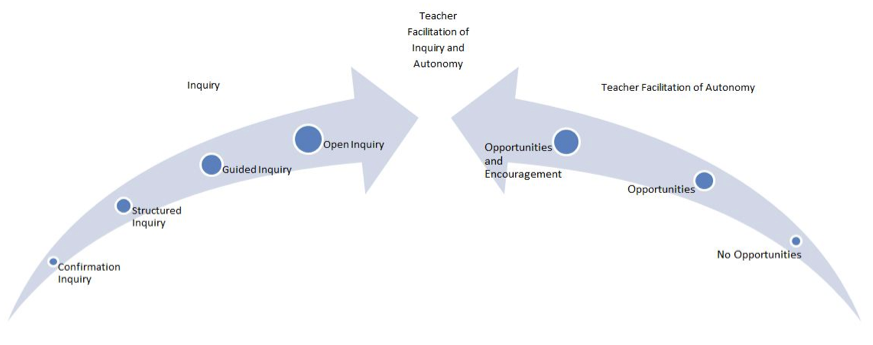
\includegraphics[width=1\textwidth]{Figure1.png}
    \caption{Model of Teacher Facilitation of Inquiry and Autonomy}
\end{figure*}

This model reconciles nicely with Crawford’s (2000) model of collaborative inquiry that suggests a spectrum of teacher involvement from lowest for discovery learning to highest for inquiry-based learning, with traditional learning in-be\-tween. In that model, the author posits that, contrary to conventional wisdom that teachers are simply “facilitators” of learning in inquiry, teachers must take highly active roles in promoting inquiry by providing authentic learning opportunities, emphasizing “grappling with data,” and developing student ownership of work.   We agree with the premise that inquiry-based learning requires tremendous preparation and active promotion of skills; however, we expand this notion and suggest that the same is true for autonomy, in which teachers must not only provide opportunities for independent work but must actively encourage it.  Simply giving students the freedom to inquire through independent work appears to foster what would most resemble “discovery learning,” but true inquiry learning requires both opportunities for independence as well as encouragement through open-ended questions, adequate time to work out problems, coaxing collaborations with other students, maintaining high expectations, and providing positive feedback.  Helping students to position themselves as scientists by engaging in authentic experiences that emulate scientists in the real world may also help students with career choices (see for example Author (2011) a challenge of particular significance to DHH students. 

\section*{CONCLUSION}

Research has suggested that DHH students tend to be dependent learners favoring teacher-centered classrooms (Lang, et al., 1999).  A related concept, that of student autonomy, has been linked to low college graduation rates for DHH students (Scherer \& Walter, 1988). When looking at the qualities that authentic scientific inquiry fosters, such as curiosity, ability to deal with uncertainty, persistence, independence and interdependence, and ability to engage in debate and discourse, it becomes clear that the habits of mind of scientists engaging in inquiry encompass many of the skills necessary for DHH students to succeed in higher education.  Autonomy, including the ability to take charge of one’s learning, evaluate and render decisions, seek out assistance when appropriate, and advocate for one’s beliefs, is intimately entwined in inquiry. This study suggests that science teachers can promote student autonomy by facilitating high quality science inquiry within a DHH student population.  While the level of inquiry may need to be scaffolded from more teacher-directed levels (confirmation and structured) to more student-driven (guided and open), the goal should be to move students toward the highest levels of inquiry and autonomy. Promoting discourse and debate as part of that inquiry may also prove particularly helpful in preparing DHH students for the inevitable social and self-advocacy challenges that arise in the college setting.  

While the findings in this study suggest avenues for fostering inquiry and autonomy in DHH science classes, there were limitations.  The small number of cases combined with the restricted time of observation provided ‘snapshots’ of the classrooms and made it difficult to generalize beyond the scope of this study.  In addition, the lack of fluency in ASL by two of us hampered our ability to interpret the students’ or teachers’ communications without an intermediary and may have caused us to misinterpret some nuances of ASL, including the use of timing and gesturing for emphasis.  We must also note that DHH students are a very heterogeneous group, representing different levels of hearing impairment, etiology of impairment (i.e. from birth or at a later point), related health impairments, and whether born to hearing or deaf parents (Marschark, et al., 2002).  These factors were not identified through our study as we were not looking at strategies that facilitate inquiry and autonomy for individual learners but rather, strategies that can be viewed as creating environments that appear to facilitate inquiry and autonomy at the classroom level. While our classrooms all utilized ASL for instruction, it is quite possible that findings in other learning environments for deaf students, such as mainstream classrooms, might differ.  Finally, our use of video, rather than being in the classrooms themselves, made it more difficult to describe the classroom set-ups and culture.  However, as stated in the methods section, great care was taken to describe the observations in detail and take other steps to ensure validity.  Remembering that case studies are not done for the purpose of generalizing, this study might be instrumental in guiding further research. 

A final consideration worth noting are some of the variables that may have contributed to the various levels of facilitation of autonomy demonstrated by our teachers.  It is perhaps not surprising that our most ‘controlling’ teacher was also the least experienced. Beginning teacher stage theory suggests that among the highest concerns of inexperienced teachers are class control, being liked by students, and being observed (Fuller\& Bown, 1975).  It is quite possible that some ‘over-facilitation’ may have been occurring due to the presence of observers and video equipment.  And while this teacher was also deaf, Serwatka, Anthony, \& Simon (1986) found no difference between instructional behaviors of deaf versus hearing teachers in their study.  Moreover, Roberson and Serwatka (2000) found no difference in deaf versus hearing teacher effectiveness as measured by standardized test scores for DHH students.  While we focused solely on teachers’ facilitation of autonomy and inquiry in the three classrooms, it should be noted that all three teachers demonstrated what appeared to be tremendous commitment to and enthusiasm for providing quality science experiences for their students. 
 
 This study suggests the need for further research in the area of science for DHH students, as there was a sobering lack of literature on this topic.  Longitudinal studies looking at DHH students’ development of science inquiry might inform the field further as to effective interventions for scaffolding inquiry.  Also, perhaps performing case studies of teachers of DHH students who facilitate inquiry well could inform the field on those best practices.  And of course, discovering if inquiry in science during the K-12 years does translate to greater autonomy and higher college graduation rates would be particularly noteworthy.   

This cross-case study suggests that DHH students have diverse learning styles and that, when given the opportunity and support to move toward open inquiry, the majority of students in these classrooms were able to do so.  This finding suggests that science may well be an ideal ‘nest’ for raising autonomous DHH students who can marshal the skills necessary to navigate higher education…to become ‘their best birds’ and fly. 

\section*{APPENDIX A}

\textbf{Theme 1 – Signs of Student Autonomy}

\begin{quote}
Code 1a – Student initiation of questioning or hypothesizing

Code 1b – Students initiating gathering of materials

Code 1c – Students proceeding through activities with limited guidance from teacher

Code 1d – Students productive in absence of teacher

Code 1e – Student advocates for ideas/\\opinions/hypotheses
\end{quote}

\textbf{Theme 2 – Teacher Facilitation of Inquiry}

\begin{quote}
Code 2a – Formal, step-wise guidance through procedure

Code 2b – Open-ended questions with wait time for student response

Code 2c – Welcoming alternative hypotheses or theories

Code 2d – Encouraging “unplanned” exploration

Code 2e – Socratic-style response to questions

Code 2f – Age/Ability appropriate scaffolding of content or process support

Code 2g – Allowing students to “fail” (i.e., make mistakes, follow “wrong” path)
\end{quote}

\textbf{Theme 3 – Interactions Among and Between Students and Teacher Related to Autonomy and Inquiry}

\begin{quote}
    
Code 3a - Evidence of collaborative problem-solving 

Code 3b – Inter-student assistance for clarification of instructions or concepts

Code 3c – Teacher encouragement for students to seek assistance from other students

Code 3d – Respectful disagreement through discourse
\end{quote}

\section*{ACKNOWLEDGMENTS}

The authors wish to thank:

The National Science Foundation (CAREER Award \#0349070)

Will Snyder and Sara Schupack for assistance with data collection and literature review

Christopher DeLuca, Mary Ellsworth, Sara Flory, and Dana Zeidler for editorial assistance 

\end{large}
\clearpage
\section*{REFERENCES}\par 

\leftskip 0.25in
\parindent -0.25in 
American Association for the Advancement of Science (1993). \textit{Benchmarks for science literacy: Project 2061}, New York, NY: Oxford University Press

American Association for the Advancement of Science (2002). \textit{New Career Paths for Students with Disabilities}. Available from \url{http://ehrweb01.aaas.org/entrypoint/pubs/}

Anderson, R. D. (2002). Reforming science teaching: What research says about inquiry. \textit{Journal of Science Teacher Education, 13}(1), 1–12.

Ary, D., Jacobs, L.C., \& Sorensen, C. (2010). \textit{Introduction to research in education}.  Belmont, CA: Wadsworth.

Barber, A. T. \& Buehl, M. M. (2012): Relations Among Grade 4 Students’ Perceptions of Autonomy, Engagement in Science, and Reading Motivation, \textit{The Journal of Experimental Education, 81}(1)22-43.

Bell, L. R, Smetana, L., \& Binns, I.  (2005) Simplifying inquiry instruction: Assessing the inquiry level of classroom activities. \textit{The Science Teacher, 72}(7)30–33.

Black, A. E., \& Deci, E. L. (2000). The effects of instructors’ autonomy support and students’ autonomous motivation on learning organic chemistry: A self-determination theory perspective. \textit{Science Education, 84}, 740–756.

Bransford, J.D., \& Donovan, S.M. (2005). Scientific inquiry and how people learn. In S.M. Donovan \&
J.D. Bransford (Eds.), \textit{How students learn: History, mathematics, and science in the classroom} (pp. 397–420). Washington, DC: The National Academies Press.

Brantlinger, E. (2005). Qualitative studies in special education. \textit{Exceptional Children, 71}(2), 195. 

Bybee, R.W. \& Van Scotter, P. (2007). Reinventing the science curriculum. \textit{Educational Leadership 64} (4) 43–47.

Cassidy, S. (2004). Learning styles: An overview of theories, models, and measures. \textit{Educational Psychology, 24}(4)419-444. 

Crawford, B.A. (2000). Embracing the essence of inquiry: New roles for science teachers. \textit{Journal of Research in Science Teaching, 37}(9)916-937.  

Deci, E. L., Schwartz, A. J., Sheinman, L., \& Ryan, R. M. (1981). An instrument to assess adults’orientations toward control versus autonomy with children: Reflections on intrinsic motivation and perceived competence. \textit{Journal of Educational Psychology, 73}, 642–650.

Denzin, N. K., \& Lincoln, Y. S. (Eds.). (2000). \textit{Handbook of qualitative research} (2nd ed.). Thousand Oaks, CA: Sage.

Dunn, R., \& Bruno, A. (1985). What does the research on learning styles have to do with Mario? \textit{Clearing House, 59}, 9-12.

Enns, C. (2009). Critical literacy: Deaf adults speak out. \textit{Exceptionality Education International, 19}(2), 3-20

Foriska, T. (1992). Breaking room tradition: Using learning styles to teach students how to learn. \textit{Schools in the Middle, 2}, 14-16.

Fuller, F. F., \& Bown, 0. H. (1975). Becoming a teacher. In K. Ryan (Ed.), \textit{Teacher education} (pp. 25-52). Chicago, IL: Chicago University Press.

Grasha, A. F. (1996). \textit{Teaching with style: Enhancing learning by understanding teaching and learning styles}. Pittsburgh, PA: Alliance Publishers.

Koestner, R., Ryan, R. M., Bernieri, F., \& Holt, K. (1984). Setting limits on children’s behavior: The differential effects of controlling versus informational styles on intrinsic motivation and creativity. \textit{Journal of Personality, 52}, 233–248.

Lang, H.G. (1994). \textit{Silence of the Spheres: The deaf experience in the history of science}. Westport, CT: Bergin \& Garvey.

Lang, H. G. (2002). Higher education for deaf students: Research priorities in the new millennium. \textit{Journal of Deaf Studies and Deaf Education, 7}(4), 267. 

Lang, H.G. \& Stinson, M.S. (1982). Career education and occupational status of deaf persons: Concepts, research, and implications. In J. Christiansen and J. Egelston-Dodd (Eds.), \textit{Socio-economic status of the deaf population}, Washington, DC: Gallaudet University. 

Lang, H., Stinson, M.S., Kavanaugh, F., Liu, Y. \& Basile, M.L. (1999). Learning styles of deaf college students and instructors' teaching emphases. \textit{Journal of Deaf Studies and Deaf Education, 4}(1), 16. 

Linn, M. C., Davis, E. A., \& Bell, P. (2004). \textit{Internet environments for science education}. Hillsdale, NJ: Erlbaum.

Livingston, S. (1997). \textit{Rethinking the education of deaf students}. Portsmouth, NH: Heinemann.

Marschark, M., \& Lang, H., \& Albertini, J.A. (2002). \textit{Educating Deaf Students: Research Into Practice}.  New York: Oxford University Press. 

Marschark, M., \& Spencer, P. E. (Eds.). (2003). \textit{Oxford handbook of deaf studies, language, and education}. New York, NY: Oxford University Press.

McIntosh R.A., Sulzen L., Reeder K., \& Kidd D.H. (1994). Making science accessible to deaf students. The need for science literacy and conceptual teaching.  \textit{American Annals of the Deaf, 139}(5), 480-4.

Molander, B. O. (2007). Ambiguity as a motor for communication—Differences between hearing and deaf students’ ways of reasoning about energy. \textit{International Journal of Educational Research, 46}(6), 327. 

National Research Council. (2012). \textit{A framework for K–12 science education: Practices, cross-cutting concepts and core ideas}. Washington, DC: National Academies Press.

National Science Foundation. (2004). \textit{Women, minorities, and persons with disabilities in science and engineering}. Washington, DC: U.S. Government Printing Office.

Niemiec, C. P. \& Ryan, R. M. (2009). Autonomy, competence, and relatedness in the classroom : Applying self-determination theory to educational practice. \textit{Theory and Research in Education, 7}(2) 133–144

Okebukola, P.A. (1986). The influence of preferred learning styles on cooperative learning in science. \textit{Science Education, 70}, 509-517.

Parasnis, I., Samar, V. J., Bettger, J. G, \& Sathe, K. (1996). Does deafness lead to enhancement of visual spatial cognition in children? \textit{Journal of Deaf Studies and Deaf Education, 1}, 145-152.

Patton, M. Q. (2002). \textit{Qualitative research and evaluation method}s (3rd ed.).Thousand Oaks, CA: Sage Publications.

Roald, I. (2002). Norwegian Deaf Teachers’ Reflections on their science education: Implications for Instruction. \textit{Journal of Deaf Studies and Deaf Education, 7} (1) 57-73. 

Roberson, L., \& Serwatka, T. S. (2000). Student perceptions and instructional effectiveness of deaf and hearing teachers. \textit{American Annals of the Deaf, 145}(3), 256–262. 

Roder B. \& Rosler, F. (2003) Memory for environmental sounds in sighted, congenitally blind and late blind adults: evidence for crossmodal compensation. \textit{International Journal of  Psychophysiology, 50}(1)27–39

Rowe, M.B. (1974). Relation of wait-time and rewards to the development of language, logic,  and fate control: Part One -- wait-time. \textit{Journal of research in science teaching, 11}(2), 81-94.

Rowe, M.B. (1986). Wait time: Slowing down may be a way of speeding up! \textit{Journal of Teacher Education 37}(1), 43 - 50.

Scherer, M.J. \& Walter, G. (1988). \textit{Student-reported satisfaction with college and reasons for college withdrawal} (Technical Report). Rochester, NY: Rochester Institute of Technology. 

Serwatka, T.S., Anthony, R.A., \& Simon, S.C. (1986), A comparison of deaf and hearing teacher effectiveness. \textit{American Annals of the Deaf 131}(5)339-343.

Shamos, M. H. (1995). \textit{The myth of scientific literacy}. New Brunswick, NJ: Rutgers University Press.

Sommer, D. (1994). Resistant texts and incompetent readers. \textit{Poetics Today, 15}(4), 523-551.  

Stefanou, C. R., Perencevich, K., DiCintio, M., \& Turner, J. C. (2004). Supporting autonomy in the classroom: Ways teachers encourage student decision making and ownership. \textit{Educational Psychologist, 39}(2), 97–110.

Sternberg, R.J., Grigorenko, E.L.,\& Zhang, L. (2008). Styles of learning and thinking matter in instruction and assessment. \textit{Perspectives on Psychological Science, 3}(6)486–506.

Stinson, M. S., \& Walter, G. G. (1997). Improving retention for deaf and hard of hearing students: What the research tells us. \textit{Journal of the American Deafness and Rehabilitation Association, 30}, 14–23.

Tharpe, A. M., Ashead, D.H., \& Rothpletz, A. M. (2002). Visual attention in children with normal hearing, children with hearing aids, and children with cochlear implants. \textit{Journal of Speech, Language, and Hearing Research, 45}(2), 403-413.

Vallerand, R. J., Fortier, M. S., \& Guay, F. (1997). Self-determination and persistence in a real-life setting: Toward a motivational model of high school dropout. \textit{Journal of Personality and Social Psychology, 72}, 1161–1176.

van Zee, E. H., Iwasyk, M., Kurose, A., Simpson, D., \& Wild, J. (2001). Student and teacher questioning during conversations about science. \textit{Journal of Research in Science Teaching, 38}(2), 159–190.

Zeidler, D.; Sadler, T.D., Simmons, M.L., \& Howes, E.V. (2005). Beyond STS: A research-based framework for socioscientific issues education. \textit{Science Education 89} (3): 357-377.

Zeidler, D.L. \& Keefer, M. (2003). The role of moral reasoning and the status of socioscientific issues in science education: Philosophical, psychological and pedagogical considerations. In D.L. Zeidler (Ed.), \textit{The role of moral reasoning on socioscientific issues and discourse in science education}. The Netherlands: Kluwer Academic Press. (pp. 7-38).
\newpage
\begin{large}

\leftskip 0in
\parindent 0in 
\section*{BIOGRAPHICAL STATEMENTS}
Sami Kahn \href{mailto:msamikahn@mail.usf.edu}{(samikahn@mail.usf.edu)} is a Presidential Doctoral Fellow in Science Education at the University of South Florida. She uses her background in law and science teaching to inform her research on inclusive science practices and socioscientific issues. She is immediate past chair of the National Science Teachers Association’s Special Needs Advisory Board, past president of Science Education for Students with Disabilities (SESD), and president of Special Science, Inc., an educational consulting firm dedicated to science for all students.  
   
Allan Feldman \href{mailto:afeldman@usf.edu}{(afeldman@usf.edu)} is a Professor of Science Education at the University of South Florida. He has been a science teacher educator for over 20 years. He has published on how inservice teachers improve their practice.  
  
Michele L. Cooke \href{mailto:cooke@geo.umass.edu}{(cooke@geo.umass.edu)} is a Professor of Geosciences at the University of Massachusetts, Amherst. She has worked with earth science teachers at schools for the Deaf since 2004 to develop innovative tectonics curriculum. 

\end{large}
\end{document}
